\documentclass[10pt,a4paper, margin=1in]{article}
\usepackage{fullpage}
\usepackage{amsfonts, amsmath, pifont}
\usepackage{amsthm}
\usepackage{graphicx}
\usepackage{float}
\usepackage{tkz-euclide}
\usepackage{tikz}
\usepackage{pgfplots}
\pgfplotsset{compat=1.13}

\usepackage{geometry}
 \geometry{
 a4paper,
 total={210mm,297mm},
 left=10mm,
 right=10mm,
 top=10mm,
 bottom=10mm,
 }
 % Write both of your names here. Fill exxxxxxx with your ceng mail address.
 \author{
  Aktolga, İlter Taha\\
  \texttt{e2236891@ceng.metu.edu.tr}
  \and
  Bolat, Burak\\
  \texttt{e2237097@ceng.metu.edu.tr}
}
\title{CENG 384 - Signals and Systems for Computer Engineers \\
Spring 2020 \\
Written Assignment 1}



\begin{filecontents}{q3.dat}
  n  xn
 -12  0
 -11  6
 -10  0  
 -9   5
 -8   0
 -7  -4
 -6  0
 -5  0
 -4  3
 -3  0
 -2 -2
 -1  0
  0  1
  1  1
  2  0
  3  0
  4 -4
  5  5
  6  6
\end{filecontents}

\begin{document}
\maketitle



\noindent\rule{19cm}{1.2pt}

\begin{enumerate}

\item 
    \begin{enumerate}
    % Write your solutions in the following items.
    \item %write the solution of q1a
    Given $z = x + yj $ and $z + 1 = j - 3\Bar{z}$ , we want to find actual value of $z$. Let's put value of $z$ form the first equation to the second equation.
    Recall that  $\Bar{z}$ which defined as $\Bar{z} = x - yj$ is the conjugate of the $z$.
    Then solve the equation in order to find $x$ and $y$ values.
    \begin{equation}
	\begin{split}
		x+yj+1 & = j - 3(x-yj)\\
		x+yj+1 & = j - 3x+3yj\\
		x+1 & = j-3x+2yj\\
		4x + 1 & = j + 2yj \\
		4x+1 -j(2y+1) & = 0\\
		x & = \dfrac{-1}{4}\\
		y & = \dfrac{-1}{2}
	\end{split}
	\end{equation}
	
	\begin{itemize}
		\item[(i)] We find $|z|^2$.
            		\begin{equation}
	       	 	\begin{split}
        				|z|^2 & = x^2 + y^2\\
        				|z|^2 & = (-1/4)^2 + (1/2)^2\\
        				|z|^2 & = 5/16
	        		\end{split}
       		 	\end{equation}
		\item[(ii)] We plot $z$ on the complex plane. \\
		\\
        \begin{tikzpicture}
        \begin{scope}[thick,font=\scriptsize]
        % Axes:
        % Are simply drawn using line with the `->` option to make them arrows:
        % The main labels of the axes can be places using `node`s:
        \draw [->] (-5,0) -- (5,0) node [above left]  {$\Re\{z\}$};
        \draw [->] (0,-5) -- (0,5) node [below right] {$\Im\{z\}$};
    
        % Axes labels:
        % Are drawn using small lines and labeled with `node`s. The placement can be set using options
        \iffalse% Single
        % If you only want a single label per axis side:
        \draw (1,-3pt) -- (1,3pt)   node [above] {$1$};
        \draw (-1,-3pt) -- (-1,3pt) node [above] {$-1$};
        \draw (-3pt,1) -- (3pt,1)   node [right] {$i$};
        \draw (-3pt,-1) -- (3pt,-1) node [right] {$-i$};
        \else% Multiple
        % If you want labels at every unit step:
        \foreach \n in {-4,...,-1,1,2,...,4}{%
            \draw (\n,-3pt) -- (\n,3pt)   node [above] {$  \n/4$};
            \draw (-3pt,\n) -- (3pt,\n)   node [right] {$(\n/4) i$};
        }
        \fi
        \end{scope}
        % The circle is drawn with `(x,y) circle (radius)`
        % You can draw the outer border and fill the inner area differently.
        % Here I use gray, semitransparent filling to not cover the axes below the circle
        % \path [draw=black] (0, 0) circle (1.414213562);
        % Place the equation into the circle:
        \draw [blue, line width=0.8] (0, 0) -- (-1, -2) node [left, blue] {$z = \dfrac{-1}{4} -\dfrac{1}{2}j$};
    \end{tikzpicture}

		
	\end{itemize}
    \item %write the solution of q1b
    Since $z^2=25j$ and $z= re^{j\theta}$. Below, we find $z$ in polar form.
    Let's start by taking square of $z$ in polar form.\\
        \begin{equation}
	\begin{split}
		z^2 & = r^2 e^{j2\theta}\\
		25j & = r^2 (cos2\theta + j sin2\theta)\\
		25j & = r^2cos2\theta + r^2jsin2\theta 
	\end{split}
	\end{equation}To satisfy last equation,there should be no real part in the right hand side. Therefore $r^2cos2\theta$ should equal to zero. For this , $cos2\theta$ should be zero.
	Recall that cosine function is zero at either $\frac{\pi}{2}$ or $\frac{3}{2}\pi$.By considering this, $2\theta$ can be $\frac{\pi}{2}$ or $\frac{3}{2}\pi$. \\
	Also note that the value of the sin function at $\frac{\pi}{2}$ is 1 and the value of the sin function at $\frac{3}{2}\pi$ is -1.If we rewrite the last equation without cosine part since it's zero:
	 \begin{equation}
	\begin{split}
		25 & = r^2 sin2\theta\\
	\end{split}
	\end{equation}
	To satisfy this equality, value of the $sin2\theta$ should be positive. Thus $2\theta$ must be $\pi/2$.
	
	From the last equation, since $sin2\theta$ is 1, r can be found as 5, because it must have positive value.\\
	
	We know $2\theta= \pi/2$ then $\theta = \pi/4$. Finally, by rewriting z in polar form, we get:
    \begin{equation}
	\begin{split}
		z & = 5 e^{\frac{\pi}{4}}\\
	\end{split}
	\end{equation}\\
	\\
	\\
    \item %write the solution of q1c
    We have given $z = \dfrac{(1+j)(1-\sqrt{3}j)}{1-j}$. Recall that polar coordinate form of a+jb is $re^{j\theta}$ where $\theta = tan^{-1}(b/a)$. We convert all the complex numbers to polar form to easily calculate. \\
    \\
    $z = \dfrac{(1+j)(1-\sqrt{3}j)}{1-j} = \dfrac{\sqrt{2}e^{j\pi/4}\times 2e^{-j\pi/3}}{\sqrt{2}e^{-j\pi/4}} = 2e^{j\pi/6}$ \\
    
	Magnitude of z is $|z|$ = 2\\
	\\Angle of z is $\pi / 6$
	\\
	
	
    \item %write the solution of q1d
    Given $ z = je^{-j\pi/2}$. To write z in polar form, we can think this equation as a product of two complex numbers.Note that, the first is in the form 0 + j. By converting the first into polar form:
     \begin{equation}
	\begin{split}
		j &= \sqrt{0^2 + 1^2} = 1 
		\end{split}
	\end{equation}
	Angle $\theta$ for the first complex number
	\begin{equation}
	\begin{split}
		tan^{-1}(\pi / 0) &= \pi /2 
		\end{split}
	\end{equation}
    we get $j= e^{j \pi/2}.$
    Then by multiplying these two complex numbers, we found z:
        \begin{equation}
	\begin{split}
		z &= (e^{j \pi/2})(e^{-j \pi/2}) \\
		z &= 1
		\end{split}
	\end{equation}
    \end{enumerate}
    
    


\item %write the solution of q2
Below is the signal for $y(t) = \frac{1}{2}x(2t - 2)$
\begin{figure}[H]
    \centering
        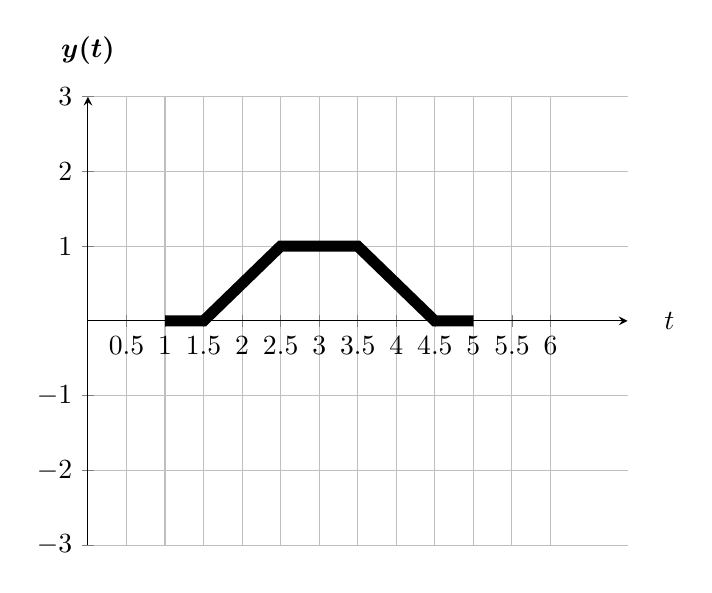
\begin{tikzpicture}[scale=1.0]
           \begin{axis}[
          axis lines=middle,
          xlabel={$t$},
          ylabel={$\boldsymbol{y(t)}$},
          xtick={0,0.5,1,1.5,2,2.5,3,3.5,4,4.5,5,5.5,6},
          ytick={-3, -2, -1, ..., 3},
          ymin=-3, ymax=3,
          xmin=0, xmax=7,
          every axis x label/.style={at={(ticklabel* cs:1.05)}, anchor=west,},
          every axis y label/.style={at={(ticklabel* cs:1.05)}, anchor=south,},
          grid,
        ]
           \path[draw,line width=4pt] (1,0) -- (3/2,0) -- (5/2,1) -- (7/2,1) -- (9/2,0) -- (5,0);
           \end{axis}
           
        \end{tikzpicture}
        \caption{$t$ vs. $y(t)$.}
        \label{fig:q222}
    \end{figure}
\item      
    \begin{enumerate}
    \item %write the solution of q3a
    Below is the signal for $x[-n] + x[2n - 1]$ 
    \begin{figure}[H]
    \centering
    \begin{tikzpicture}[scale=2.0] 
      \begin{axis}[
          xshift=7cm,
          enlargelimits=0.05,
          axis lines=middle,
          xlabel={$n$},
          ylabel={$\boldsymbol{x[-n]+x[2n-1]}$},
          xtick={-12,-11,-10,-9, -8, ..., 6},
          ytick={-4, -3, -2, -1, ..., 6},
          ymin=-5, ymax=6,
          xmin=-12, xmax=6,
          every axis x label/.style={at={(ticklabel* cs:1.05)}, anchor=west,},
          every axis y label/.style={at={(ticklabel* cs:1.05)}, anchor=south,},
          grid,
        ]
        \addplot [ycomb, black, thick, mark=*] table [x={n}, y={xn}] {q3.dat};
      \end{axis}
    \end{tikzpicture}
    \caption{$n$ vs. $x[-n]+x[2n-1]$.}
    \label{fig:q3}
\end{figure}
    \item %write the solution of q3b
    Expression of $x[-n] + x[2n-1] $ in terms of unit step functions:\\
    
            \begin{equation}
	\begin{split}
		x[-n] + x[2n-1] &=  6 \delta[n+11] + 5\delta[n+9] -4\delta[n+7] + 3\delta[n+4]-2\delta[n+2]+\delta[n]+\\ & \delta[n-1]-4\delta[n-4]+5\delta[n-5]+6\delta[n-6]  \\
		\end{split}
	\end{equation}
    \end{enumerate}

\item 
    \begin{enumerate}
    \item %write the solution of q4a
    Define $y[n] = sin[\dfrac{5\pi}{8} n]$, so that it is a shifted and scaled version of $7sin[\dfrac{5\pi}{8} n - \dfrac{2\pi}{3}]$.
    If this equation is periodic, then it holds:
    \begin{equation}
        sin[\dfrac{5\pi}{8}n] = sin[\dfrac{5\pi}{8}(n+N)]\\
    \end{equation}
    \begin{equation}
    \begin{split}
        \dfrac{5\pi}{8}N = 2\pi m\\
        \dfrac{5\pi}{16} = \dfrac{m}{N}\\
        N_1 = 16\\
    \end{split}
    \end{equation}
    Same for the $2cos[\dfrac{2\pi}{3}n]$, define $z[n] = cos[\dfrac{2\pi}{3}n]$\\
    If this equation is periodic, then it holds:
    \begin{equation}
        \begin{split}
            cos[\dfrac{2\pi}{3}n] = cos[\dfrac{2\pi}{3}(n+N)]\\
        \end{split}
    \end{equation}
    \begin{equation}
        \begin{split}
            \dfrac{2\pi}{3}N = 2\pi m\\
            \dfrac{1}{3} = \dfrac{m}{N}\\
            N_2 = 3\\
        \end{split}
    \end{equation}
    Since two parts of the signal are periodic, the signal is periodic. It's fundamental period is $N_0 = lcs(3,16) = 48$\\
    \item %write the solution of q4b
    Following the approach applied in part a gives:\\
    \begin{equation}
        \begin{split}
            cos[5n] = cos[5(n+N)]\\
            5N = 2\pi m\\
            \dfrac{5}{2\pi} = \dfrac{m}{N}\\
        \end{split}
    \end{equation}
    There is no m and N integer pairs that satisfy equation.
    \item %write the solution of q4c
    If the signal is periodic, then:\\
    \begin{equation}
        \begin{split}
            5\pi T = 2\pi\\
            T_0 = \dfrac{2}{5}
        \end{split}
    \end{equation}
    \item %write the solution of q4d
    As first step, represent j in polar form:\\
    \begin{equation}
        j = e^{j\frac{\pi}{2}}
    \end{equation}
    Then given equation becomes:
    \begin{equation}
        \begin{split}
            e^{j\frac{\pi}{2}}e^{j2t} = e^{j(2t+\dfrac{\pi}{2})}\\
        \end{split}
    \end{equation}
    If the signal is periodic then:
    \begin{equation}
        \begin{split}
            e^{j(2t+\dfrac{\pi}{2})} = e^{j(2(t+T)+\dfrac{\pi}{2})}\\
            e^{j2T} = 1\\
            cos(2T) + j sin(2T) = 1\\
            T_0 = \pi\\
        \end{split}
    \end{equation}
    $T_0 = \pi$ to eliminate imaginary part and receive 1 as real part.
    \end{enumerate}

\item %write the solution of q5
Given signal in Figure 1 is neither even nor odd.
We know that $x(t) = Even\{x(t)\} + Odd\{x(t)\} $ and we can find even part:
 \begin{equation}
	\begin{split}
		Even\{x(t)\} &= \frac{1}{2}(x(t)+x(-t)) \\
		\end{split}
	\end{equation}
and odd part as:
 \begin{equation}
	\begin{split}
		 Odd\{x(t)\} &= \frac{1}{2}(x(t)-x(-t)) \\
		\end{split}
	\end{equation}

So $\text{Ev\{x[n]\}}$ can be drawn as: \\
\begin{figure}[H]
    \centering
        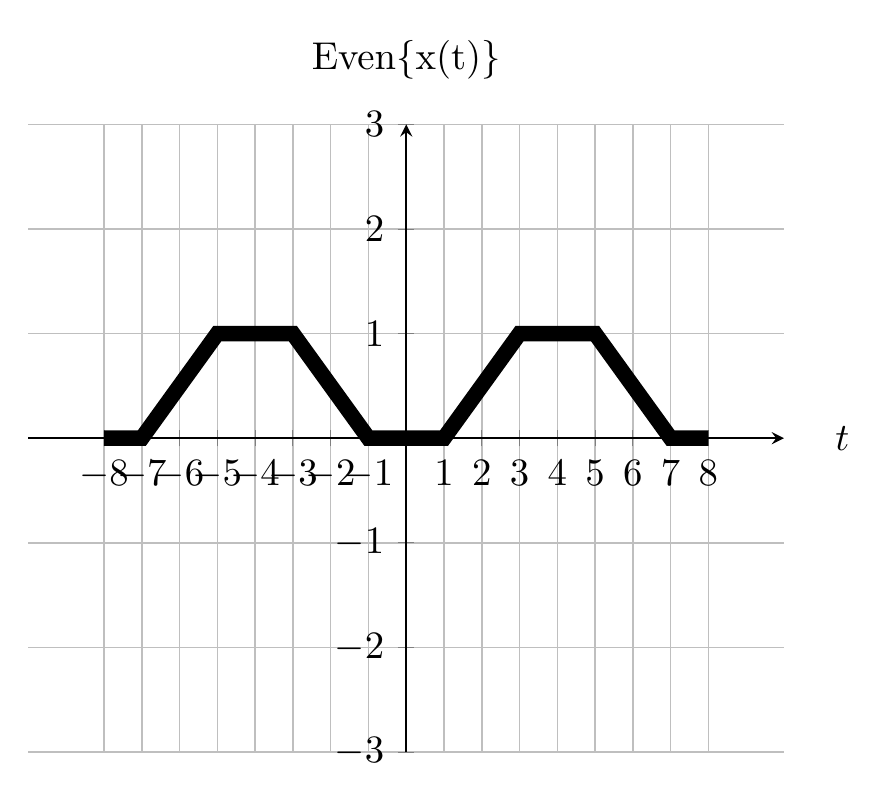
\begin{tikzpicture}[scale=1.4]
           \begin{axis}[
          axis lines=middle,
          xlabel={$t$},
          ylabel={$\text{Even\{x(t)\}}$},
          xtick={-8,-7,-6,-5,-4,-3,-2, ..., 8},
          ytick={-3, -2, -1, ..., 3},
          ymin=-3, ymax=3,
          xmin=-10, xmax=10,
          every axis x label/.style={at={(ticklabel* cs:1.05)}, anchor=west,},
          every axis y label/.style={at={(ticklabel* cs:1.05)}, anchor=south,},
          grid,
        ]
           \path[draw,line width=4pt] (-8,0) -- (-7,0) -- (-5,1) -- (-3,1) -- (-1,0) -- (1,0) -- (3,1) -- (5,1) -- (7,0) -- (8,0);
           \end{axis}
        \end{tikzpicture}
        \caption{$t$ vs. $\text{Even\{x(t)\}}$.}
        \label{fig:q2}
    \end{figure}

and $\text{Odd\{x(t)\}}$ can be drawn as: \\
\begin{figure}[H]
    \centering
        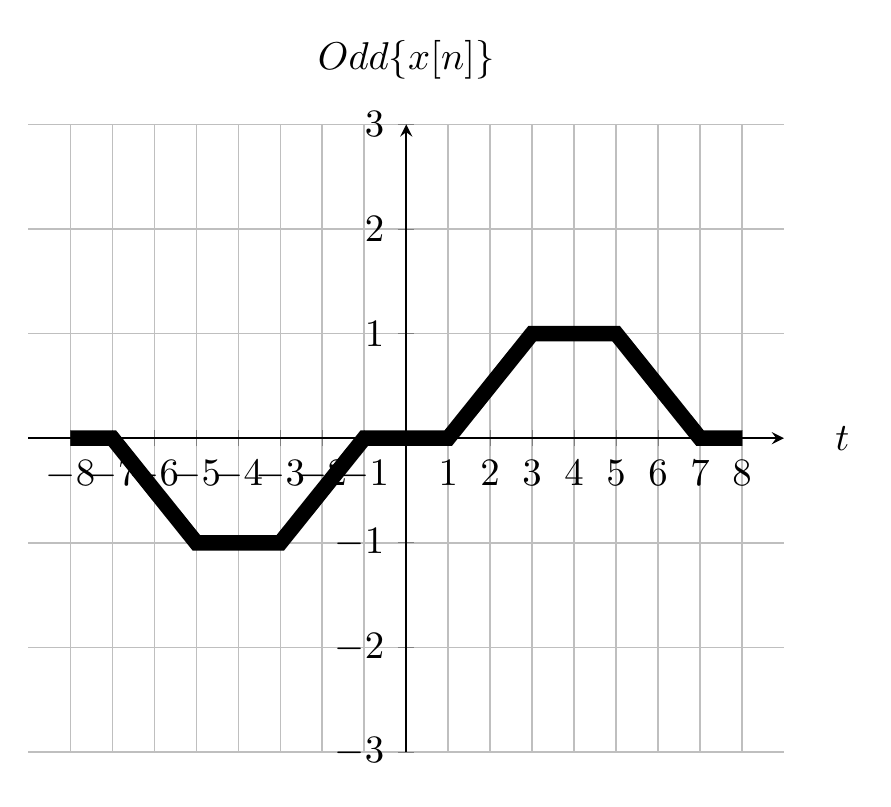
\begin{tikzpicture}[scale=1.4]
           \begin{axis}[
          axis lines=middle,
          xlabel={$t$},
          ylabel={${Odd\{x[n]\}}$},
          xtick={-8,-7,-6,-5,-4,-3,-2, ..., 8},
          ytick={-3, -2, -1, ..., 3},
          ymin=-3, ymax=3,
          xmin=-9, xmax=9,
          every axis x label/.style={at={(ticklabel* cs:1.05)}, anchor=west,},
          every axis y label/.style={at={(ticklabel* cs:1.05)}, anchor=south,},
          grid,
        ]
           \path[draw,line width=4pt] (-8,0) -- (-7,0) -- (-5,-1) -- (-3,-1) -- (-1,0) -- (1,0) -- (3,1) -- (5,1) -- (7,0) -- (8,0);
           \end{axis}
        \end{tikzpicture}
        \caption{$t$ vs. $\text{Odd\{x(t)\}}$.}
        \label{fig:q22}
    \end{figure}


\item 
    \begin{enumerate}
    \item %write the solution of q6a
    Expression of x(t) in terms of unit functions:
        \begin{equation}
	\begin{split}
		x(t) &= u(t-1)-(3u(t-3)) +(4u(t-4)) \\
		\end{split}
	\end{equation}
    \item %write the solution of q6b 
    To find derivative of x(t), we look for changes in the graph.
    At points where t=1, t=3 and t=4, u(t) is  discontinuous and consequently is formally not differentiable. We can, however, interpret  by considering an approximation to the unit step which rises from the value 0 to the value 1 in a  short time interval of length $\Delta$. The unit step, of course, changes values instantaneously and thus can be thought of as an idealization of $u_{\Delta}(t)$ for very short $\Delta$.In other words u(t) is the limit of $u_{\Delta}(t)$ as $\Delta$ $\rightarrow 0$ \\
    
    Graph of the $\frac{dx(t)}{dt}$ can be seen below. \\
\begin{figure}[H]
        \centering
        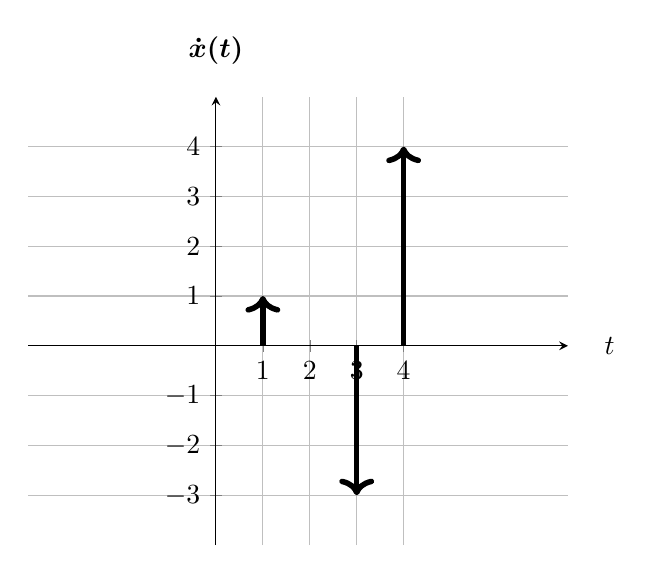
\begin{tikzpicture}[scale=1.0]
           \begin{axis}[
          axis lines=middle,
          xlabel={$t$},
          ylabel={$\boldsymbol{\dot x(t)}$},
          xtick={0, 1, ..., 4},
          ytick={-3,-2, -1, 0, 1, 2,3,4},
          ymin=-4, ymax=5,
          xmin=-4, xmax=7.5,
          every axis x label/.style={at={(ticklabel* cs:1.05)}, anchor=west,},
          every axis y label/.style={at={(ticklabel* cs:1.05)}, anchor=south,},
          grid,
        ]
           \path[draw,line width=2pt,->] (1,0) -- (1,1);
           \path[draw,line width=2pt,->] (3,0) -- (3,-3);
           \path[draw,line width=2pt,->] (4,0) -- (4,4);
           \end{axis}
        \end{tikzpicture}
        \caption{Graph of $\frac{dx(t)}{dt}$.}
        \label{fig:q6}
    \end{figure}
    \end{enumerate}

\end{enumerate}
\end{document}

    \item %write the solution of q4d


